

%L'apparato sperimentale attualmente in uso ai LNS-INFN nell'ambito della Fase~2 del progetto NUMEN, costituito principalmente dallo spettrometro MAGNEX e dal Ciclotrone Superconduttore K800, viene brevemente illustrato nella prima parte di questo capitolo.
L'apparato sperimentale attualmente in uso ai LNS-INFN nell'ambito della Fase~2 del progetto NUMEN è costituito principalmente dallo spettrometro MAGNEX e dal CS.
Poiché la descrizione di tale apparato non costituisce l'argomento primario del presente lavoro di tesi, nella parte iniziale del capitolo vengono discusse soltanto le sue caratteristiche principali, rimandando alla vasta letteratura sul tema per informazioni più dettagliate (ad esempio~\cite{cavallaro:epja12, carbone:epja12, cappuzzello:epja16, cunsolo:epjst07}).

%Nella prima parte di questo capitolo vengono illustrate le principali caratteristiche dell'apparato sperimentale attualmente in uso ai LNS-INFN nell'ambito della Fase~2 del progetto NUMEN.
%Nella seconda parte viene descritta la configurazione dell'apparato adottata in occasione del test sui telescopi SiC-CsI svolto ad Aprile 2018, sottolineando le differenze rispetto a quella consueta.
(\textcolor{red}{Sistemare questa parte})Nella seconda parte \textcolor{red}{si parla} del test sui telescopi SiC-CsI svolto ad Aprile~2018, esponendone le motivazioni, descrivendo la configurazione dell'apparato adottata e sottolineandone le differenze rispetto a quella consueta.


\section{\iflanguage{italian}{Lo spettrometro magnetico MAGNEX}{MAGNEX magnetic spectrometer}}

Lo spettrometro magnetico MAGNEX è un dispositivo ottico a grande accettanza costituito da un quadrupolo per la focalizzazione sull'asse verticale, seguito da un dipolo per la dispersione sul piano orizzontale.
Grazie alle sue peculiarità,  MAGNEX riesce ad offrire, in un angolo solido molto grande e in un ampio range energetico, un'ottima risoluzione in energia, angolo e massa.
Ciò lo rende uno strumento ideale per l'analisi di eventi caratterizzati da sezioni d'urto molto basse, come è già stato dimostrato in~\cite{cappuzzello:epja16,pereira:plb12,oliveira:jpg13}.
Inoltre, esso consente di effettuare misure fino a zero gradi, comprendendo, dunque, la regione angolare di massimo interesse per lo studio del DCE.

La caratteristica che rende MAGNEX uno strumento unico è l'implementazione di una innovativa tecnica di ricostruzione delle traiettorie degli ioni, che consente di correggere le inevitabili aberrazioni originate dalla grande accettanza del dispositivo.
Dunque, a differenza di altri spettrometri magnetici, per MAGNEX è importante determinare non soltanto il punto di impatto sul piano focale ma anche la traiettoria completa. Ciò significa che è necessario misurare quattro parametri: una coppia, chiamata $(x_{foc}, y_{foc})$, individua il punto di impatto, l'altra, indicata con $(\theta_{foc}, \phi_{foc})$, si riferisce rispettivamente all'angolo orizzontale e a quello verticale.
%Nel paragrafo successivo verrà esplicato in che modo vengono misurati tali parametri.
Il modo in cui tali parametri vengono misurati sarà esplicato nel paragrafo successivo.

In Figura~\ref{fig:magnex} è mostrata una foto di MAGNEX, in cui è possibile notare, andando da sinistra verso destra, la camera di scattering, il quadrupolo, il dipolo e il~FPD (\textcolor{red}{Aggiungere le scritte sull'immagine}).

\begin{figure} [!t]
	\centering
	\includegraphics[width=\textwidth, keepaspectratio]{Grafici/magnex_etichette.png}
	\caption{Lo spettrometro magnetico MAGNEX.} \label{fig:magnex}
\end{figure}



%\clearpage 

\subsection{\iflanguage{italian}{L'attuale rivelatore di piano focale}{The present Focal Plane Detector}} \label{sez:fpd}

\begin{figure} [!p]
	\centering
	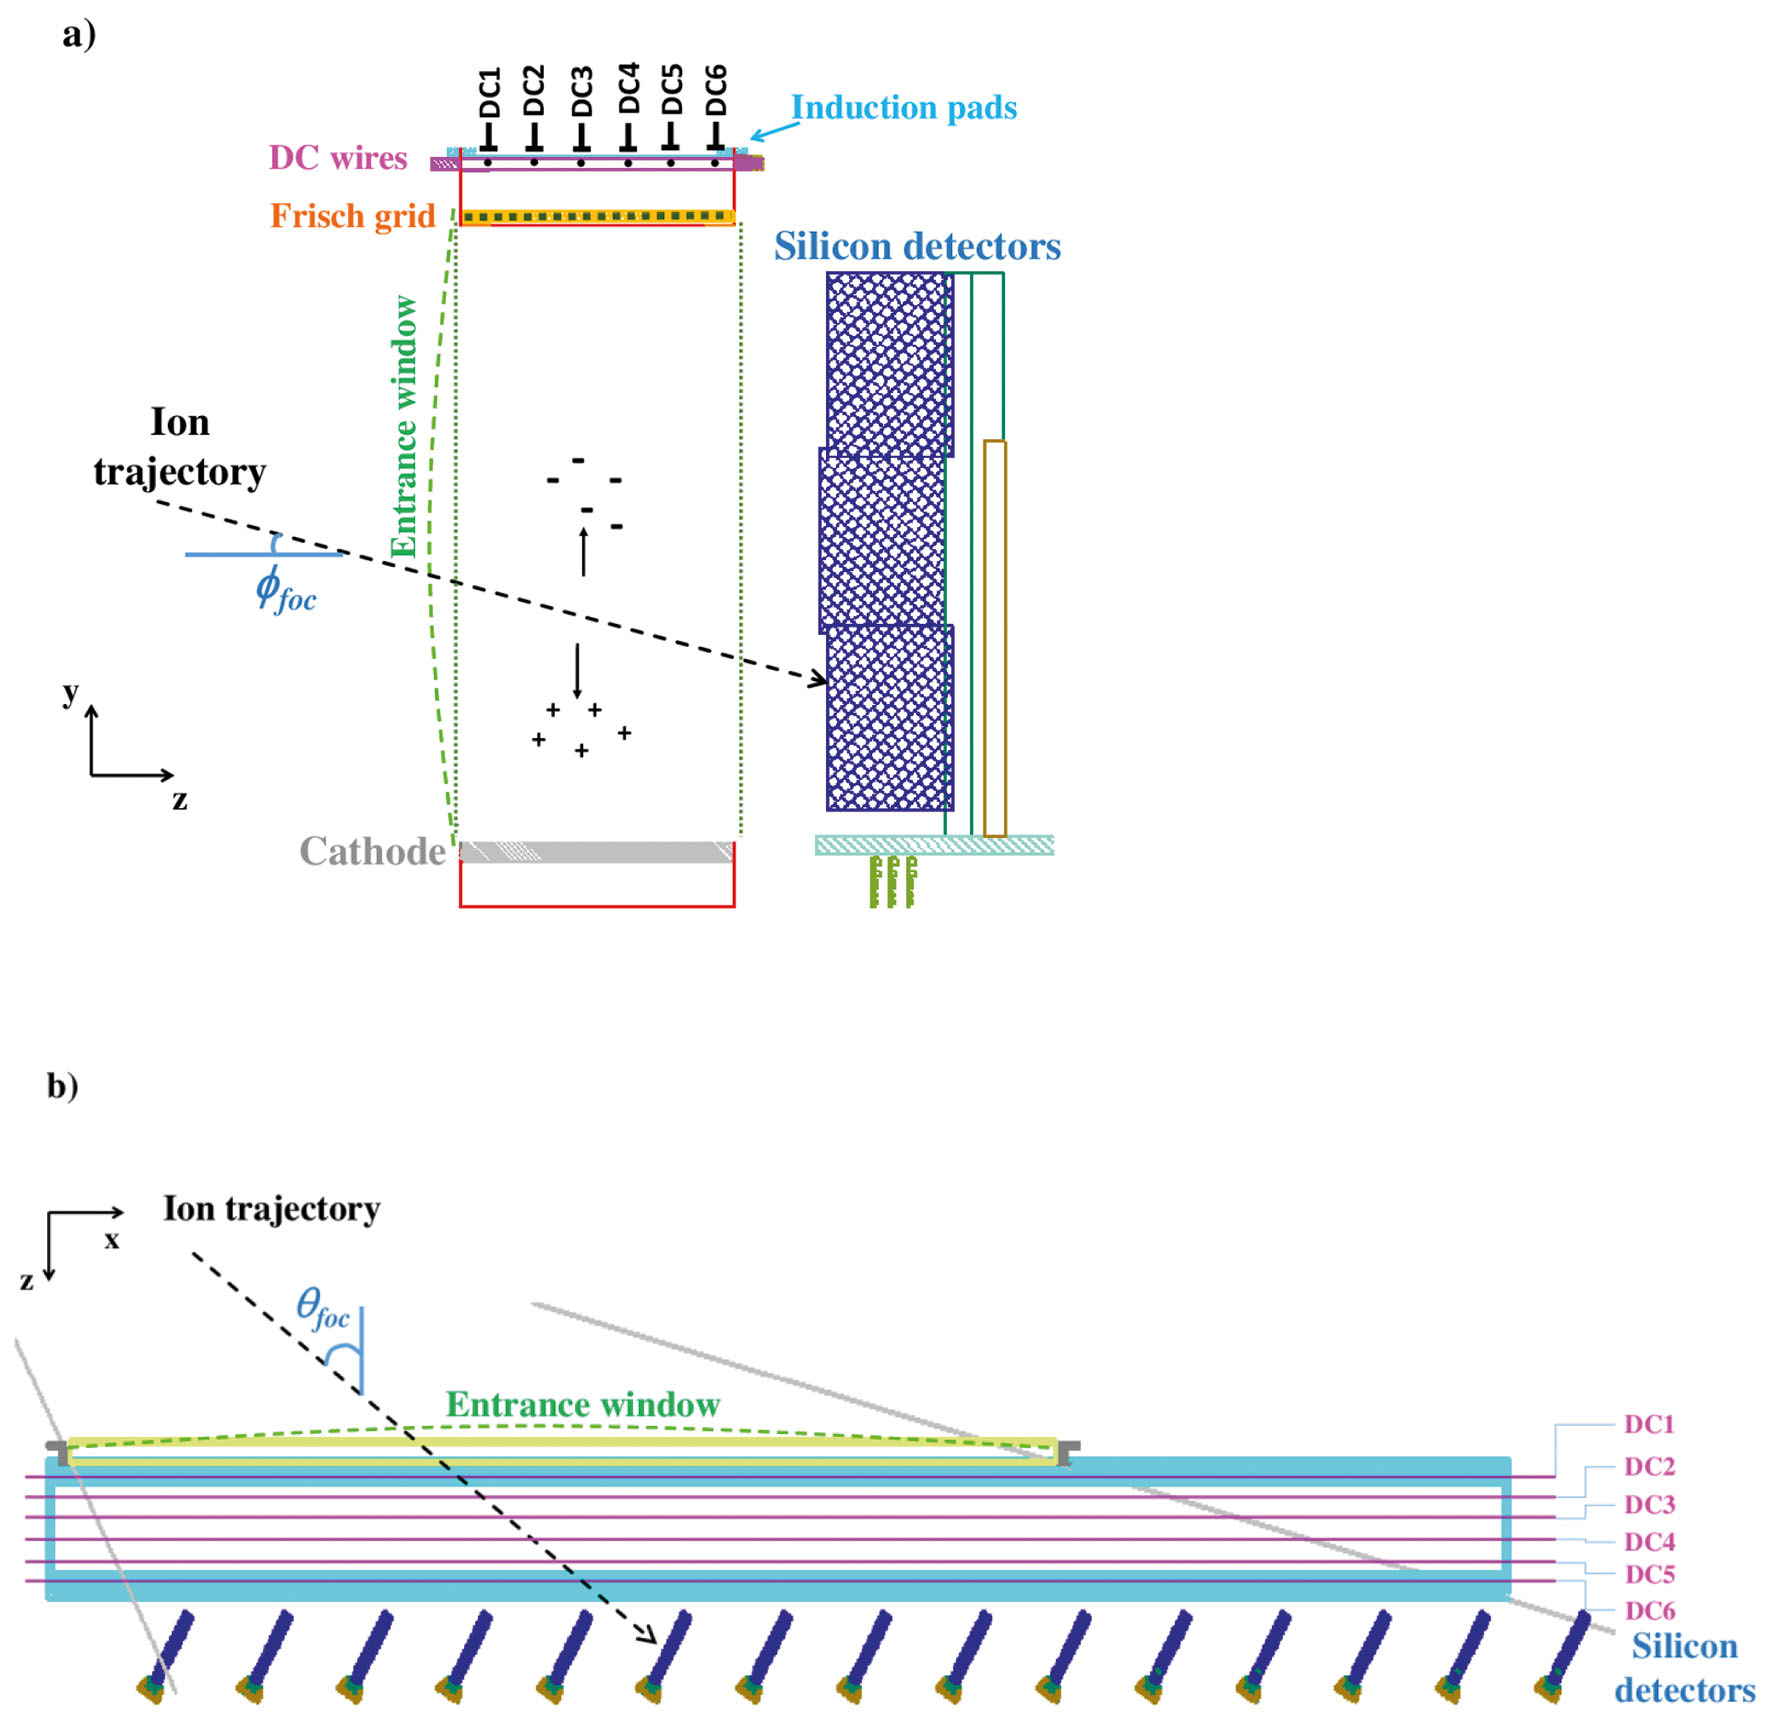
\includegraphics[width=\textwidth, keepaspectratio]{Grafici/fpd.png}
	\caption{Rappresentazione schematica del FPD: a) vista laterale; b) vista dall'alto. Figura tratta da~\cite{cappuzzello:epja18}.} \label{fig:fpd}
\end{figure}

L'attuale FPD di MAGNEX, la cui rappresentazione schematica è riportata in Figura~\ref{fig:fpd}, è un sistema di rivelazione ibrido, costituito da un tracciatore a gas a bassa pressione e da un muro di rivelatori al silicio.
Esso è posizionato a 1.91~m dall'uscita del dipolo e, al fine di minimizzare gli effetti dovuti alle aberrazioni cromatiche~\cite{cunsolo:nima01}, è inclinato di 59.2\textdegree{} rispetto ad un piano perpendicolare all'asse ottico.
%Una finestra di mylar spessa 1.5~$\mu$m è utilizzata per contenere il gas, solitamente costituito da N35 isobutano, segnando l'ingresso nel volume attivo.
L'ingresso nel volume attivo è segnato da una finestra di mylar spessa 1.5~$\mu$m, la quale è utilizzata per contenere il gas, solitamente costituito da N35 isobutano.



%Il tracciatore a gas è formato da un sistema di sei fili al tungsteno placcati in oro, posti al di sotto di un anodo segmentato in pad. 
%Il tracciatore a gas lavora secondo il principio tipico delle camera a deriva.
%Il tracciatore a gas è essenzialmente una camera a deriva, in cui un sistema misto di fili e pad consente la misura dei quattro parametri necessari.
%Il tracciatore a gas, che consente la ricostruzione tridimensionale della traiettoria degli ioni, è formato da sei fili al tungsteno, indicati con DC\ped{\textit{i}}, e da un anodo segmentato in pad. 
%Al di sopra di ciascun filo si trova una fila di 224 pad
%Il tracciatore a gas è essenzialmente una camera a deriva, in cui un sistema costituito da sei fili (DC\ped{\textit{i}}) e da un anodo segmentato in pad consente la misura dei quattro parametri necessari per la ricostruzione tridimensionale della traccia.
%In particolare, al di sopra di ciascun filo è presente una fila di pad, le quali sono orientate parallelamente all'asse ottico.
Il tracciatore a gas, che consente la ricostruzione tridimensionale della traiettoria degli ioni, è formato da sei fili proporzionali (DC\ped{\textit{i}}) e da un anodo segmentato in sei file di pad, disposti in modo che sopra ogni filo ci sia una fila di pad.
I fili, sfruttando il principio di lavoro delle camere a deriva, danno una misura di sei posizioni verticali ($Y_i$), mentre le pad permettono di determinare sei posizioni orizzontali ($X_i$).
%Una griglia di Frisch è posta al di sotto dei fili, in quanto questi vengono anche utilizzati per misurare l'energia persa dagli ioni nel gas.
Dal momento che i fili vengono anche utilizzati per misurare l'energia persa dagli ioni nel gas, una griglia di Frisch è posta al di sotto di essi.




Il muro di rivelatori al silicio è formato da 60 pad, organizzate in 20 colonne da 3 rivelatori ciascuna. (\textcolor{red}{Aggiungo qualche dettaglio in più?})
%Ogni pad ha un'area attiva di $70 \times 50$~mm\ap{2} ed è spessa 500~$\mu$m, sufficienti per fermare i prodotti di reazioni nel range energetico di interesse. 
Essi vengono utilizzati per fermare gli ioni, misurandone l'energia residua e producendo il segnale di trigger per l'acquisizione. 

Quando una particella carica, attraversando la finestra di mylar, entra nel volume attivo, perde energia nel gas producendo coppie elettrone-ione positivo, le quali, sotto l'effetto di un campo elettrico uniforme, migrano rispettivamente verso la griglia di Frisch e il catodo. 
%mentre gli elettroni diffondono verso la griglia di Frisch, con una velocità che per questi ultimi è di circa $3 - 5 $~cm/$\mu$s. 
%La presenza di un campo elettrico costante provoca 
%La velocità di deriva tipica degli elettroni è di $3 - 5 $~cm/$\mu$s
Dopo aver attraversato la griglia, gli elettroni giungono in prossimità dei fili DC\ped{\textit{i}}, dove, a causa dell'elevato campo elettrico, danno luogo alla moltiplicazione a valanga. 
%La carica prodotta, proporzionale all'energia persa dalla particella nel gas, induce sulle pad una distribuzione di carica, della quale si calcola il baricentro. Questa operazione avviene per le sei file di pad, in modo tale che ai sei baricentri corrispondono sei misure di posizioni orizzantali $X_i$.
Alle tensioni e pressioni utilizzate, la carica secondaria prodotta genera un segnale proporzionale all'energia persa dalla particella nel gas. 
Poiché ciò avviene per ciascuno dei sei fili, si hanno sei segnali di perdita di energia, indicati con~$\Delta E_i$.

La stessa valanga induce sulle pad una distribuzione di carica, di cui si calcola, tramite un apposito software, il centro di gravità. Anche in questo caso l'operazione si ripete per le sei file di pad, così che vengono estratte sei misure di posizioni orizzontali~$X_i$.
A questo punto, effettuando un fit lineare sulle sei posizioni~$X_i$, si ottengono $x_{foc}$ e $\theta_{foc}$ rispettivamente dall'intercetta e dal coefficiente angolare della retta.

Superata la regione del tracciatore, la particella carica arriva al muro dei rivelatori al silicio, dove si ferma producendo un segnale proporzionale alla sua energia residua~$E_{resid}$. 
Lo stesso segnale viene utilizzato per calcolare l'intervallo di tempo impiegato dagli elettroni primari prodotti nel gas per raggiungere i fili DC\ped{\textit{i}}. 
%Dal momento che tale intervallo è proporzionale allo spazio percorso, si ottengono così sei misure di posizioni verticali~$Y_i$, dalle quali, grazie ad un fit lineare, si ricavano $y_{foc}$ e $\phi_{foc}$ in maniera analoga a quanto visto per $x_{foc}$ e $\theta_{foc}$.
Dal momento che la velocità di deriva è costante, tale intervallo di tempo è direttamente proporzionale allo spazio percorso. Si ottengono, dunque, sei misure di posizioni verticali~$Y_i$, dalle quali, grazie ad un fit lineare, si ricavano $y_{foc}$ e $\phi_{foc}$ in maniera analoga a quanto visto per $x_{foc}$ e $\theta_{foc}$.

È bene ricordare che, nelle camere a deriva a fili, la maggior parte del segnale è originata dal moto degli ioni positivi e non degli elettroni.
Di conseguenza, a causa della minore velocità degli ioni, tale tipologia di rivelatori può tipicamente sostenere rate dell'ordine di pochi~kHz. 
Questo aspetto, che costituisce una delle principali limitazioni all'intensità del fascio tollerabile dall'attuale FPD, deve essere superato nell'ottica della Fase~4. 
%Nasce da qui l'esigenza di sostituire l'attuale tracciatore con un sistema in grado di lavorare con un rate elevato di ioni pesanti. 
%Nasce da qui l'esigenza di sostituire l'attuale
Esso costituisce, dunque, uno dei principali motivi alla base del cambiamento del sistema di rivelazione degli eiettili con uno in grado di lavorare con un rate elevato di ioni pesanti. 
%Da qui trae origine la grande opera di cambiamento del sistema di rivelazione degli eiettili con uno in grado di lavorare con un rate elevato di ioni pesanti.



\section{\iflanguage{italian}{Il futuro rivelatore di piano focale}{Future Focal Plane Detector}}

%Il FPD previsto per la Fase~4 del progetto NUMEN manterrà una struttura simile a quella attuale, in quanto consisterà di un sistema di tracciamento tridimensionale a gas e di un muro di rivelatori per la PID.


%Il FPD previsto per la Fase~4 del progetto NUMEN consisterà di un tracciatore tridimensionale e di un muro di telescopi $\Delta E - E$.

Il FPD previsto per la Fase~4 del progetto NUMEN, pur mantenendo una struttura simile a quella attuale, dovrà fare uso di tecnologie innovative, molte delle quali sono ancora in fase di sviluppo.
Esso consisterà di un sistema di tracciamento tridimensionale a gas e di un muro di rivelatori per la~PID.


Il nuovo tracciatore, al momento in fase di sviluppo, dovrà garantire la misura ad alta risoluzione dei quattro parametri $ \left(  x_{foc}, y_{foc}, \theta_{foc}, \phi_{foc}  \right)$ necessari per la ricostruzione della traiettoria in condizioni di alti rate di particelle incidenti. 
%Esso sarà fondamentalmente costituito da tre parti: una regione di deriva per gli elettroni prodotti dalla ionizzazione, un elemento per la moltiplicazione degli elettroni e una scheda segmentata di readout.
Esso sarà fondamentalmente costituito da tre parti:
\begin{itemize}
	\item[--] una regione di deriva per gli elettroni prodotti dalla ionizzazione;
	\item[--] un elemento per la moltiplicazione degli elettroni, ovvero un Micro-Pattern Gas Detector (MPGD);
	\item[--] una scheda segmentata di readout.
\end{itemize}

Una particella carica incidente, dopo aver attraversato la finestra di mylar per il contenimento del gas, produce lungo la sua traiettoria una traccia di coppie elettrone-ione positivo. 
%Il campo elettrico uniforme fra il catodo e l'elemento per la moltiplicazione guida gli elettroni
%Il campo elettrico uniforme fra catodo e anodo guida gli elettroni primari verso l'elemento di moltiplicazione
Sotto l'azione del campo elettrico uniforme presente fra catodo e anodo, gli elettroni primari si muovono con velocità costante nella regione di deriva fino a raggiungere il MPGD.
Analogamente a quanto visto nel Paragrafo~\ref{sez:fpd}, dalla misura del tempo di deriva degli elettroni primari è possibile estrarre l'informazione sulla posizione e sull'angolo verticali.
Giunti al MPGD, gli elettroni primari danno origine ad una moltiplicazione a valanga, che risulta nella formazione di un jet elettronico. 
Tale jet viene guidato dal campo elettrico verso la scheda segmentata di readout, dove induce su delle strip un impulso di carica. 
Di conseguenza, note le strip coinvolte, è possibile misurare la posizione e l'angolo orizzontali. 





Dopo aver attraversato il tracciatore a gas, la particella carica raggiunge il muro per la PID, che, come anticipato nel Paragrafo~\ref{sez:sistema_identif_part}, sarà costituito da una matrice di telescopi $\Delta E - E$ basati sulla tecnologia SiC-CsI.
%Poiché la simulazione svolta per questo lavoro di tesi verte principalmente su tale argomento,
Poiché l'argomento principale del presente lavoro di tesi consiste nella simulazione di tale sistema di identificazione, per maggiore chiarezza si è preferito discutere dei telescopi nel paragrafo successivo.

La scelta della tecnologia da utilizzare per il MPGD è oggi orientata verso le Thick-GEM, che, grazie alla loro capacità di sostenere rate fino al MHz/mm\ap{2}, sono adatte agli scopi di NUMEN.
Tuttavia, diverse delle condizioni in cui questo tipo di rivelatori sono abitualmente utilizzati non sono attuabili per NUMEN. 
In primo luogo, le Thick-GEM sono tipicamente utilizzate con gas a pressione atmosferica, mentre il FPD opera solitamente a pressioni di alcune decine di mbar.
Inoltre, esse spesso sono utilizzate per particelle in condizioni di Minimum Ionizing Particle, mentre gli ioni di interesse per NUMEN saranno ben lontani da tali energie.
%In aggiunta, dal momento che diversi tipi di ioni raggiungono il rivelatore, il tracciatore deve avere ...
Dunque, sebbene incoraggianti risultati siano stati recentemente ottenuti, questa soluzione richiede un'intensa attività di sviluppo.


Una rappresentazione schematica del futuro FPD è mostrata in Figura~\ref{fig:nuovo_fpd}, dove sono raffigurate anche le superfici equipotenziali calcolate con il codice Poisson-Superfish~\cite{superfish:87}: le linee quasi parallele indicano che nella regione di deriva il campo elettrico è piuttosto uniforme.


Un prototipo di dimensioni ridotte, mostrato in Figura~\ref{fig:castelletto}, è stato realizzato per individuare le migliori soluzioni in termini di geometria, tensioni applicate, MPGD ed elettronica.




\begin{figure} [!t]
	\centering
	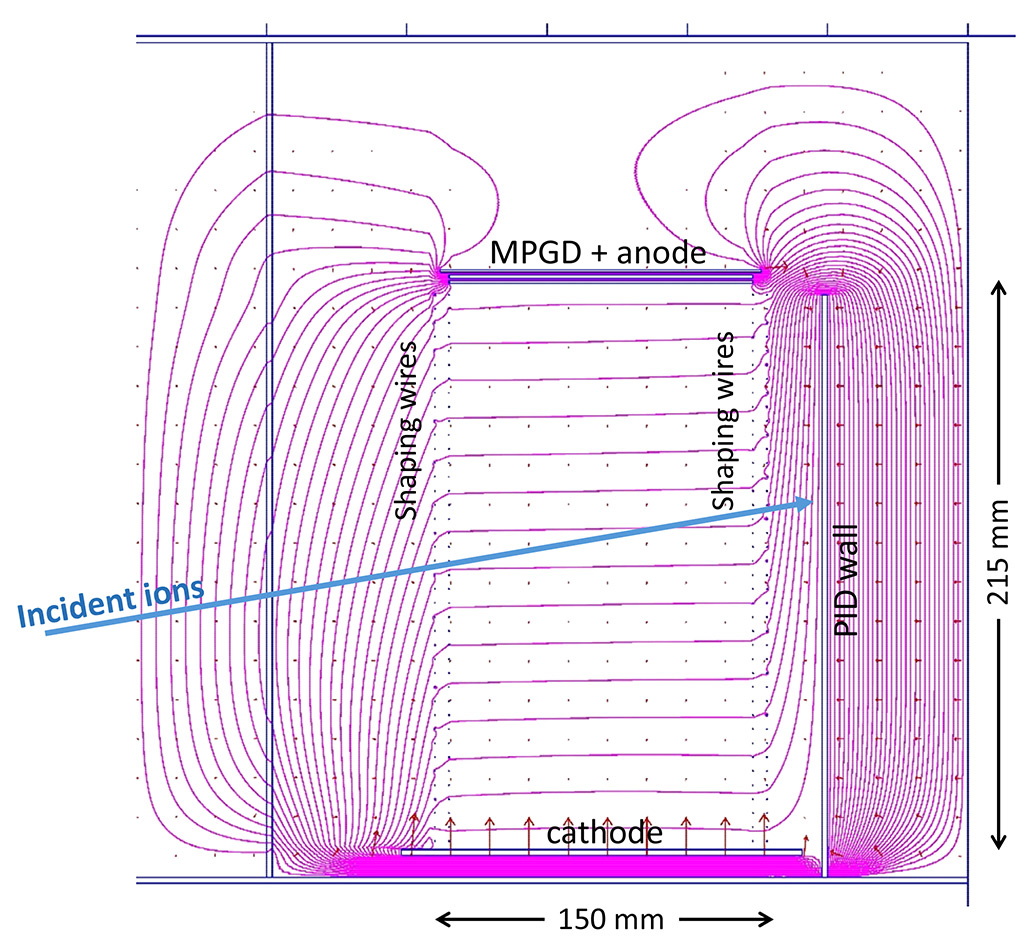
\includegraphics[scale=0.25]{Grafici/nuovo_fpd.png}
	\caption{Rappresentazione schematica del previsto FPD. Le linee magenta indicano le superfici equipotenziali, mentre le frecce mostrano il corrispondente campo elettrico. Figura tratta da~\cite{cappuzzello:epja18}.} \label{fig:nuovo_fpd}
\end{figure}

\begin{figure} [!p]
	\centering
	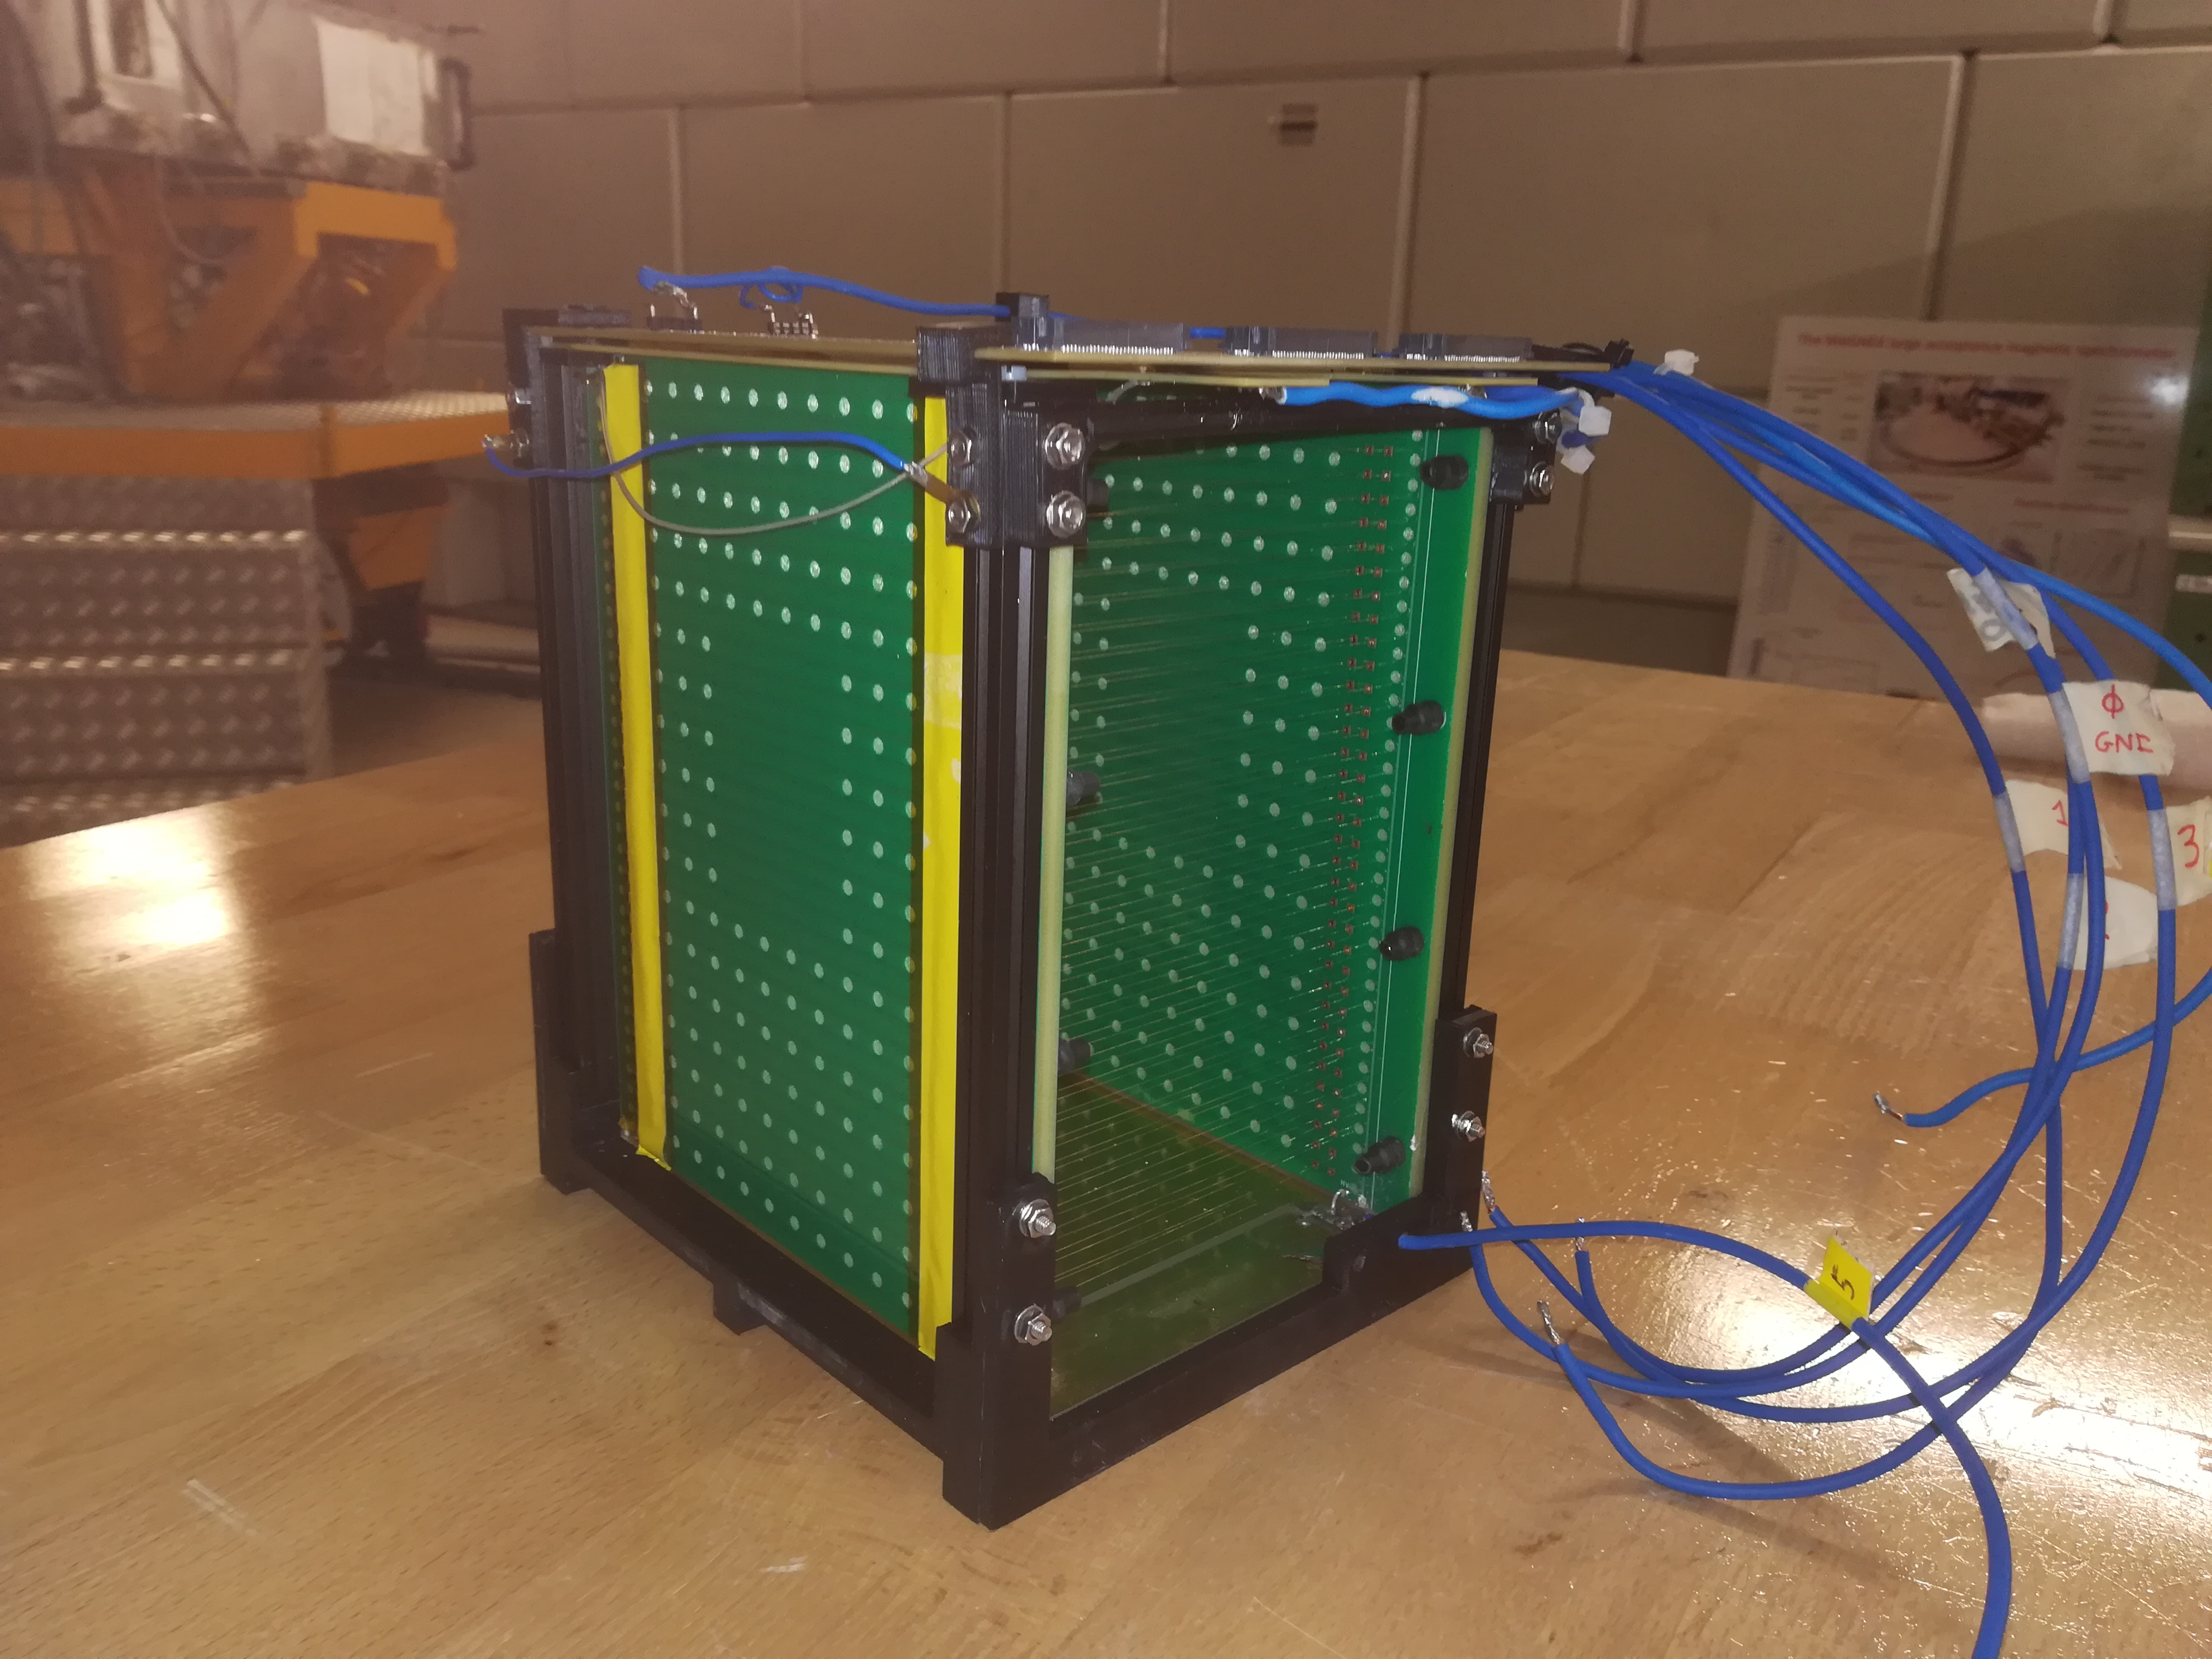
\includegraphics[width=\textwidth, keepaspectratio]{Grafici/castelletto3.jpg}
	\caption{Rappresentazione schematica del previsto FPD. Le linee magenta indicano le superfici equipotenziali, mentre le frecce mostrano il corrispondente campo elettrico. Figura tratta da~\cite{cappuzzello:epja18}.} \label{fig:castelletto}
\end{figure}




%\section{\iflanguage{italian}{Il test sui telescopi SiC-CsI}{Experimental setting for the test}}
\section{\iflanguage{italian}{I telescopi SiC-CsI}{SiC-CsI telescope detectors}}

%Ad Aprile 2018 è stato svolto un test sui primi due prototipi di telescopi SiC-CsI, allo scopo di confrontarne la risposta con il sistema attualmente utilizzato.
%Ad Aprile 2018 è stato svolto un test sui primi due prototipi di telescopi SiC-CsI, allo scopo di valutarne la risposta, confrontandola con quella del sistema attualmente utilizzato.


%Dopo aver realizzato 
%Per verificare se la risposta di un telescopio formato da uno stadio $\Delta E$ al SiC seguito da un cristallo di CsI poteva garantire prestazioni di identificazione degli ioni confrontabili con quelle accessibili con l'attuale apparato, è stato svolto un test per una durata complessiva di cinque giorni.
%Dal momento che tali rivelatori non sono ancora uno standard nel mondo della fisica ma rappresentano una tecnologia nuova, è stato svolto un test per verificare se le loro prestazioni possono soddisfare le esigenze di NUMEN.

%Come illustrato nel Paragrafo~\ref{sez:sistema_identif_part}, i rivelatori al SiC sono stati scelti nell'ambito del progetto per assolvere al ruolo di sistema di PID
%Sono stati, dunque, assemblati due telescopi SiC-CsI, di cui si è studiata la risposta in termini di PID.

%Come illustrato nel Paragrafo~\ref{sez:sistema_identif_part}, i rivelatori al SiC sono stati scelti nell'ambito del progetto per identificare i prodotti di reazione

Quando si studiano le reazioni fra ioni pesanti, l'identificazione in numero atomico, massa e carica dei prodotti di reazione è una componente indispensabile, che, a seconda delle esigenze, viene eseguita adoperando vari metodi.
%Una delle tecniche più diffuse prevede l'utilizzo di telescopi $\Delta E - E$.
Come anticipato nel Paragrafo~\ref{sez:sistema_identif_part}, il progetto NUMEN ha individuato come possibile soluzione per la PID in condizioni di alti rate di particelle incidenti l'utilizzo di telescopi $\Delta E - E$ in cui il primo stadio è un rivelatore al SiC, mentre il secondo è uno scintillatore allo CsI.
Vediamo più in dettaglio queste due tipologie di rivelatori.






%Il fascio utilizzato nel test era costituito da \ce{^{20}Ne}, mentre i bersagli erano \ce{^{197}Au} e \ce{^{12}C}







%\subsection{\iflanguage{italian}{I telescopi SiC-CsI}{SiC-CsI telescope detectors}}

\subsection{\iflanguage{italian}{I rivelatori al carburo di silicio}{Silicon carbide detectors}}


%I dispositivi al SiC costituiscono oggi una promettente realtà nel campo dei rivelatori per la fisica, 
Grazie alle sue interessanti proprietà, il SiC costituisce oggi una promettente realtà nel campo della realizzazione di rivelatori per la fisica, configurandosi come una potenziale alternativa al silicio nelle applicazioni che richiedono una grande resistenza alle radiazioni.
%La larghezza della sua gap, quasi tripla rispetto a quella del silicio, se da un lato aumenta l'energia media per la produzione di una coppia elettrone-lacuna, dall'altro riduce il numero di portatori di carica generati per agitazione termica, mantenendo, dunque, un ottimo rapporto segnale-rumore.
La larghezza della sua gap, quasi tripla rispetto a quella del silicio, se da un lato riduce il numero di portatori di carica generati per agitazione termica, dall'altro aumenta l'energia media per la produzione di una coppia elettrone-lacuna. 
Ciò significa che, a parità di energia, una particella incidente su un rivelatore al SiC crea un terzo dei portatori di carica prodotti in un rivelatore al silicio, generando, dunque, un segnale di ampiezza inferiore.
%Dunque, i rivelatori al SiC generano segnali di ampiezza inferiore rispetto a quelli dei rivelatori al silicio.
Tuttavia, gli ioni pesanti di interesse per NUMEN dovrebbero generare un numero elevato di coppie elettrone-lacune, così che l'ampiezza del segnale dovrebbe essere sufficientemente grande.
Inoltre, i rivelatori al SiC hanno un ottimo rapporto segnale-rumore anche a temperature piuttosto alte, mentre i rivelatori al silicio hanno, in alcuni casi, bisogno di un sistema di raffreddamento.
Recenti test~\cite{tudisco:sensors18} hanno dimostrato che con un rivelatore da 100~$\mu$m di spessore è possibile ottenere una risoluzione energetica dello 0.8\%~FWHM per le particelle $\alpha$ dell'\ce{^{241}Am} a 5486~keV.


Come la maggior parte dei rivelatori a semiconduttore, i rivelatori al SiC sono costituiti da una giunzione p-n, polarizzata inversamente per aumentare l'estensione della regione svuotata e per migliorare l'efficienza di raccolta dei portatori di carica.
Quando una particella carica attraversa il rivelatore, perde energia generando coppie elettrone-lacuna, le quali, in presenza di un campo elettrico, si muovono verso gli elettrodi, producendo un segnale elettrico proporzionale all'energia depositata.

%La resistenza alle radiazioni dei rivelatori al SiC è stata indagata sia attraverso simulazioni Monte Carlo sia per mezzo di test sperimentali. 
Poiché la resistenza alle radiazioni è l'aspetto di maggiore importanza per la scelta dei dispositivi da utilizzare per NUMEN, alcune simulazioni Monte Carlo sono state implementate allo scopo di darne una stima nel caso dei rivelatori al SiC. 
In Figura~\ref{fig:sic_simul_resist_radiaz} (a sinistra) sono riportati i risultati della produzione di vacanze generata da protoni e \ce{^{18}O} in un rivelatore da 100~$\mu$m.
Come si può notare, i difetti causati dagli ioni di ossigeno sono due ordini di grandezza maggiori di quelli indotti dai protoni.
Un comportamento simile si osserva anche sulla corrente inversa, mostrata in Figura~\ref{fig:sic_simul_resist_radiaz} (a destra). Sebbene aumenti di diversi ordini di grandezza dopo alte dosi di irradiazione, essa può essere ancora tollerabile, essendo cinque ordini di grandezza inferiore a quella del silicio.

La resistenza alle radiazioni di rivelatori al SiC di piccole dimensioni ($2 \times 2$~mm\ap{2}, 30~$\mu$m di spessore) è stata analizzata in un test in cui i dispositivi erano irraggiati con ioni pesanti~\cite{raciti:npa10}. 
I risultati hanno dimostrato che tali rivelatori sono in grado di sostenere fluenze dell'ordine di $10^{14}$  $\mbox{ioni}/\mbox{cm}^2$, soddisfacendo il principale requisito di NUMEN.

\begin{figure} [!t]
	\centering
	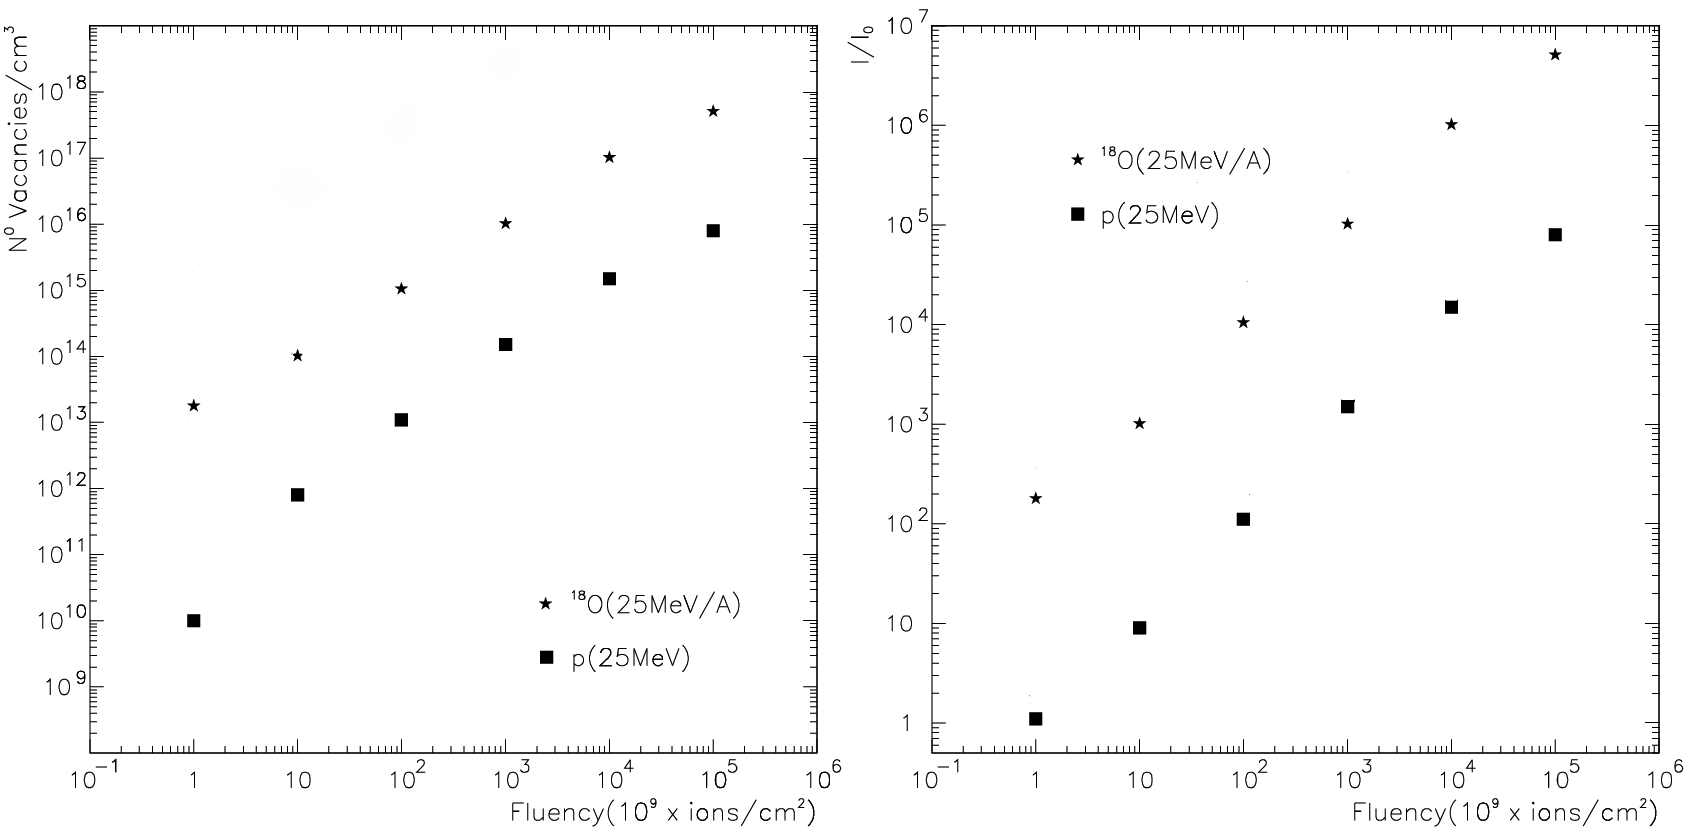
\includegraphics[width=\textwidth, keepaspectratio]{Grafici/sic_simul_resist_radiaz.png}
	\caption{ Simulazioni Monte Carlo del numero di dislocamenti (a sinistra) e della corrente inversa (a destra) generati in un rivelatore al SiC da 100~$\mu$m in funzione della fluenza di protoni e \ce{^{18}O}. Figura tratta da~\cite{cappuzzello:epja18}.} \label{fig:sic_simul_resist_radiaz}
\end{figure}



%Gli attuali limiti tecnologici alla produzione di rivelatori al SiC sono legati alla capacità di controllare le dimensioni dell'area attiva e lo spessore dei dispositivi, dal momento che essi vengono realizzati tramite crescita epitassiale su un substrato di SiC.
Gli attuali limiti tecnologici alla produzione di rivelatori al SiC sono legati alla capacità di fabbricare dispositivi con area attiva e spessori relativamente grandi, dal momento che essi vengono realizzati tramite crescita epitassiale su un substrato di SiC.
%Ciò comporta anche la presenza di una regione in cui la ... ZONA PARZIALMENTE VIVA .... NON SO BENE COME INTRODURLA
Inoltre, la presenza di tale substrato può rappresentare un problema ai fini della rivelazione, in quanto costituisce uno strato morto in cui le particelle perdono energia senza che questa possa essere misurata o possono perfino fermarsi.
%Tali problematiche sono state tenute in considerazione nella simulazione svolta per questo lavoro di tesi, la quale ne ha valutato l'impatto sulle performance del previsto sistema di rivelazione. 
La simulazione svolta per questo lavoro di tesi ha tenuto in considerazione tali limiti e problematiche, valutandone l'impatto sulle performance del previsto sistema di rivelazione e suggerendo le migliori specifiche tecniche ai fini del progetto. 






%I due prototipi di rivelatori al SiC utilizzati nel test sono mostrati in Figura~\ref{fig:sic}; essi avevano caratteristiche differenti: uno, chiamato \emph{SiC~A}, aveva un'area attiva non segmentata di $10 \times 10$~mm\ap{2}, con uno spessore di 10~$\mu$m ed uno strato morto di 100~$\mu$m; l'altro, indicato con \emph{SiC~B}, aveva un'area attiva segmentata in quattro pad, ciascuna di $5 \times 5$~mm\ap{2}, con uno spessore di 100~$\mu$m ed un strato morto di 350~$\mu$m.





%I due prototipi di rivelatori al SiC utilizzati nel test presentavano caratteristiche differenti: in primo luogo avevano spessore diversi, poiché uno era spesso 10~$\mu$m, mentre l'altro 100~$\mu$m.



\subsection{\iflanguage{italian}{Gli scintillatori allo ioduro di cesio}{Caesium iodide scintillation detector}}





%\subsection{\iflanguage{italian}{I telescopi SiC-CsI}{SiC-CsI telescope detectors}}
I rivelatori a scintillazione, detti anche \emph{scintillatori}, sono tra i più diffusi strumenti per la rivelazione delle particelle.
%Il loro principio di funzionamento è basato sul fatto che quando una particella carica attraversa uno scintillatore vengono emessi fotoni. 
%Il loro principio di funzionamento è basato sull'emissione di luce di scintillazione da parte di certi materiali quando attraversati da una particella carica
Il loro principio di funzionamento è il seguente: quando una particella carica attraversa uno scintillatore, eccita gli atomi o le molecole del materiale, i quali si diseccitano emettendo fotoni. 
La luce prodotta, proporzionale all'energia depositata nel cristallo, viene raccolta e trasformata in segnale elettrico da appositi sensori, come i fotomoltiplicatori o i fotodiodi.
Dal momento che l'energia media necessaria per la creazione di un fotone è circa trenta volte superiore a quella richiesta per la produzione di una coppia elettrone-lacuna in un semiconduttore, la risoluzione energetica tipica degli scintillatori è peggiore di quella dei rivelatori a semiconduttore.
%, con valori tipicamente compresi tra $1 \div 3 \%$.
%I due rivelatori al SiC sono stati assemblati insieme ai due scintillatori allo CsI mostrati in Figura~\ref{fig:csi}. 
%Fra le tipologie più diffuse di scintillatori, lo ioduro di cesio occupa uno dei posti più importanti.

Molti materiali possono produrre luce di scintillazione, differenziandosi per resa in luce, linearità e tempi di decadimento, laddove la resa in luce esprime il numero di fotoni prodotti per unità di energia depositata, la linearità descrive il rapporto di proporzionalità fra la resa in luce e l'energia depositata, il tempo di decadimento indica il tempo necessario per l'emissione di luce dopo il deposito di energia.
Uno dei materiali più diffusi per la realizzazione di rivelatori a scintillazione è lo CsI attivato al Tl, indicato solitamente come CsI(Tl). 
%Dal momento che possiede una fra le maggiori rese in luce e una notevole malleabilità, viene spesso impiegato nella rivelazione sia di particelle cariche sia di raggi gamma.
Dal momento che possiede una fra le maggiori rese in luce e una notevole malleabilità, negli ultimi cinquant'anni ha trovato un largo utilizzo negli esperimenti sia di fisica nucleare sia di fisica particellare, venendo impiegato nella rivelazione di particelle cariche o di raggi gamma.


%La resistenza alle radiazioni dei cristalli di CsI è stata largamente studiata
%Innumerevoli test sono stati condotti per valutare la resistenza alle radiazioni dei cristalli di CsI(Tl), 
%Uno degli aspetti che hanno contribuito alla diffusione dello CsI(Tl) (nel seguito indicato come CsI) è la sua resistenza alle radiazioni, che è stata oggetto di innumerevoli test~\cite{beylin:nima04}. I risultati sono concordi nell'affermare che, sebbene ci siano fluttuazioni legate alla purezza e alle dimensioni dei cristalli, la resa in luce non dovrebbe subire variazioni significative alle intensità di fascio che verranno utilizzate per NUMEN.
%
%Innumerevoli studi sono stati condotti per valutare la resistenza alle radiazioni dello CsI(Tl) (nel seguito indicato come CsI) utilizzando  
%La resistenza alle radiazioni dello CsI(Tl) (nel seguito indicato come CsI) è stata oggetto di innumerevoli test in cui i cristalli venivano irraggiati con raggi gamma o con elettroni.
Uno degli aspetti che ha contribuito alla diffusione dello CsI(Tl) (nel seguito indicato come CsI) è la sua resistenza alle radiazioni, che è stata oggetto di innumerevoli test in cui i cristalli venivano irraggiati con raggi gamma o con elettroni~\cite{beylin:nima04, zhu:nima98}.
%I risultati sperimentali danno incoraggianti prospettive di sopravvivenza per i cristalli alle intensità di fascio che verranno utilizzate per NUMEN.
%I risultati sono concordi nell'affermare che, sebbene ci siano fluttuazioni legate alla purezza e alle dimensioni dei cristalli, la resa in luce non dovrebbe subire variazioni significative alle intensità di fascio che verranno utilizzate per NUMEN.
Tuttavia, dal momento che in letteratura non sono stati trovati dati sperimentali riguardo la sua resistenza agli ioni pesanti, la collaborazione NUMEN ha svolto un test sottoponendo un cristallo di CsI di $ 1 \times 1$~cm\ap{2} ad un fascio di \ce{^{14}N} a 65~MeV/u, per una fluenza totale di circa $10^{12}$~particelle/cm\ap{2}, equivalente a circa un anno di esperimento (\textcolor{red}{giusto?}).
Alla fine dell'irraggiamento, il cristallo non presentava danni visibili e la sua resa in luce non mostrava variazioni.
Supportati da questi incoraggianti risultati, la scelta di utilizzare lo CsI sembra promettere le capacità di resistenza alle radiazioni necessarie per NUMEN.






%\clearpage

%\section{\iflanguage{italian}{La configurazione dell'apparato sperimentale nel test}{Experimetal apparatus setting}}
\section{\iflanguage{italian}{Il test sperimentale sui telescopi}{Telescope detectors experimental test}}

% ******** QUESTA ERA LA PARTE CHE SECONDO ME VA BENE PER INTRODURRE IL TEST
Ad Aprile 2018 i primi due prototipi di rivelatori al SiC per il progetto NUMEN sono stati completati e resi disponibili dalla \textcolor{red}{ST-Microelectronics} (\textcolor{red}{giusto?}). Dal momento che tali rivelatori non sono ancora uno standard nel mondo della fisica ma rappresentano una tecnologia di frontiera, è stato condotto un test per analizzarne la risposta nelle condizioni sperimentali tipiche della Fase~2 di NUMEN, valutandone la capacità di PID nella regione di interesse per NUMEN e confrontandola con quella accessibile con l'attuale apparato. 
%Come illustrato nel Paragrafo~\ref{sez:sistema_identif_part}, i rivelatori al SiC sono stati scelti nell'ambito del progetto come stadio~$\Delta E$ di un telescopio SiC-CsI per l'identificazione in numero atomico dei prodotti di reazione. Lo scopo principale del test era, dunque, valutare la capacità di PID di questo sistema nella regione di interesse per NUMEN, confrontandola con quella accessibile con l'attuale apparato.


Il test è stato svolto utilizzando un fascio di~\ce{^{20}Ne} a 20~MeV/u, incidente su \ce{^{197}Au} o \ce{^{12}C}, laddove i due bersagli avevano funzioni differenti: il primo serviva per la localizzazione dello scattering elastico, il secondo per favorire la formazione dei prodotti di reazione di interesse.
%, ovvero quella dell'O, del F e del Ne.











I due prototipi di rivelatori al SiC utilizzati nel test sono mostrati in Figura~\ref{fig:sic}: come è possibile notare, essi differivano innanzitutto per la segmentazione dell'area attiva, in quanto uno, chiamato \emph{SiC~A}, era costituito da un'unica pad, mentre l'altro, indicato con \emph{SiC~B}, era suddiviso in quattro regioni. 
%Inoltre, mentre il SiC~A aveva un'area attiva di $10 \times 10$~mm\ap{2}, il SiC~B presentava 
%I due telescopi SiC-CsI utilizzati nel test
Entrambi i rivelatori avevano un'area attiva complessiva di $10 \times 10$~mm\ap{2}, laddove ogni pad del SiC~B aveva un'estensione di $5 \times 5$~mm\ap{2}.
%Un'ulteriore differenza riguardava gli spessori dei due rivelatori: mentre il SiC~A era spesso 10~$\mu$m con 100~$\mu$m di strato morto, il SiC~B aveva uno spessore di 100~$\mu$m con 350~$\mu$m di .
Un'ulteriore differenza riguardava lo spessore della regione attiva dei due rivelatori: per il SiC~A era di 10~$\mu$m, mentre per il SiC~B misurava 100~$\mu$m.
Infine, entrami i rivelatori avevano uno strato morto che, mentre per il SiC~A era spesso 100~$\mu$m, per il SiC~B aveva uno spessore di~350~$\mu$m.

In occasione del test si è scelto di utilizzare soltanto due delle quattro pad del SiC~B, le quali sono state cortocircuitate tra loro in modo tale che il rivelatore avesse una superficie sensibile di $10 \times 5$~mm\ap{2}.


\begin{figure} [!t]
	\centering
	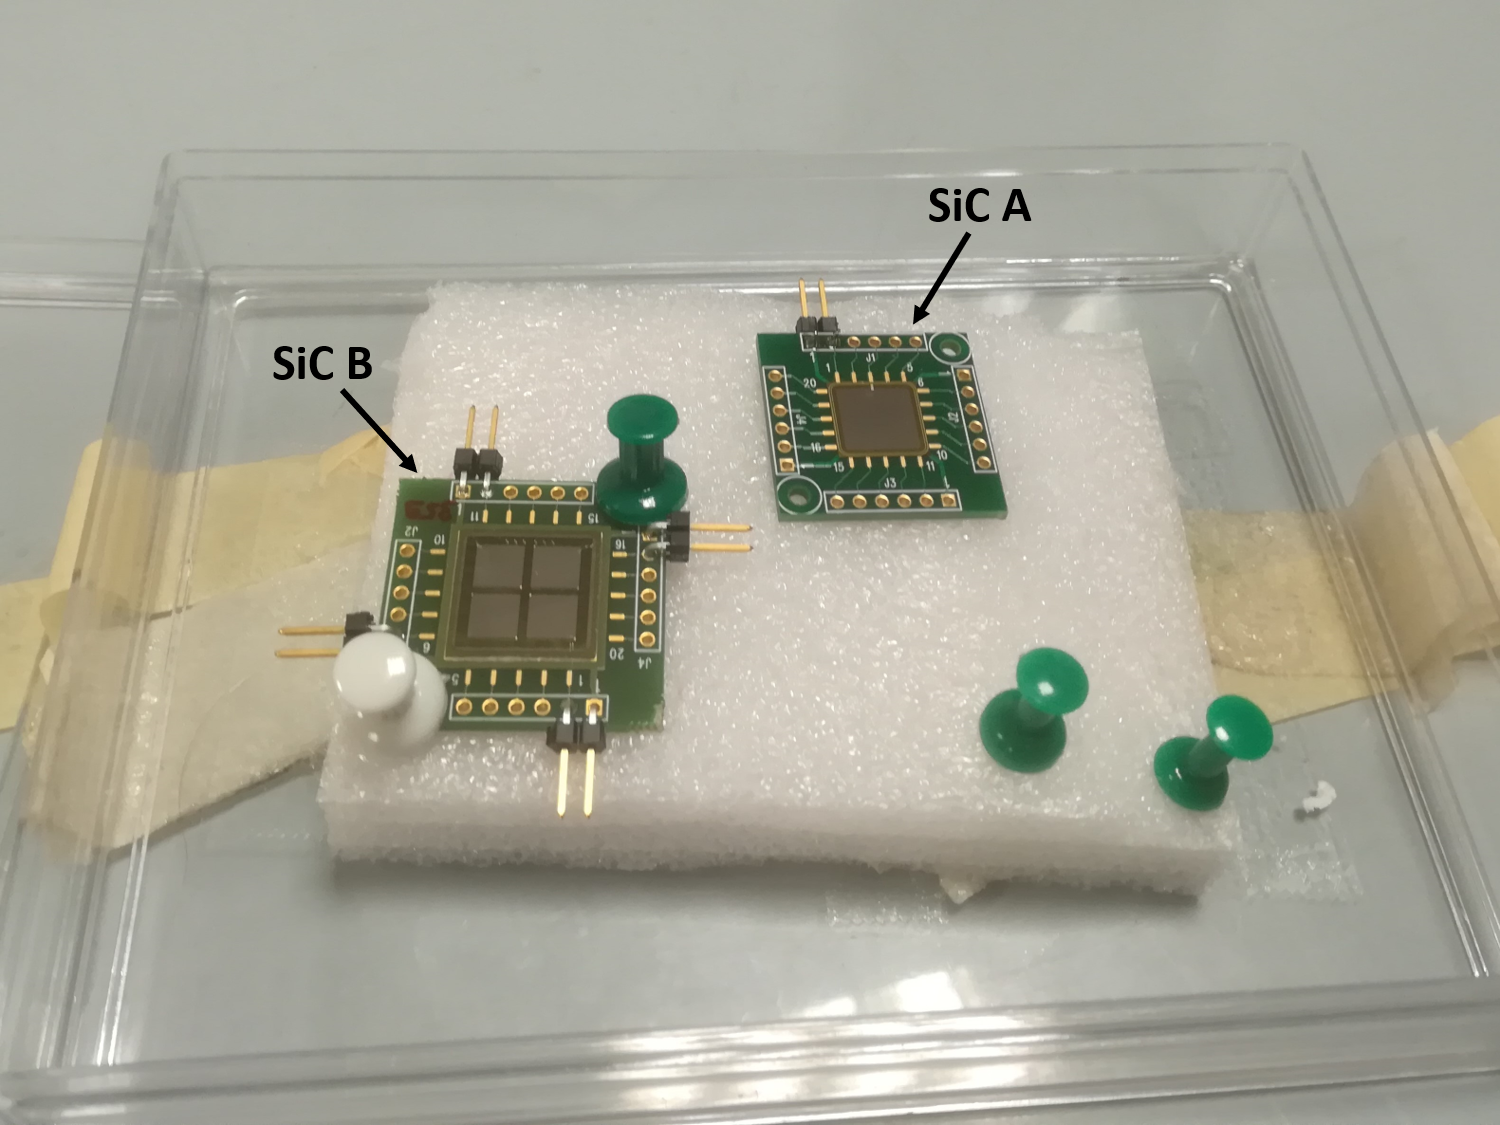
\includegraphics[width=\textwidth, keepaspectratio]{Grafici/sic_etichette.png}
	\caption{I rivelatori al carburo di silicio (SiC) utilizzati nel test: a sinistra il \emph{SiC~B}, a destra il \emph{SiC~A}.} \label{fig:sic}
\end{figure}





In occasione del test sono stati utilizzati due scintillatori allo CsI, i quali sono mostrati in Figura~\ref{fig:csi}
Questi avevano dimensioni differenti: uno (\emph{CsI~A}) era grande $1 \times 1$~cm\ap{2}, l'altro (\emph{CsI~B}) era suddiviso in quattro regioni da $1.5 \times 1.5$~cm\ap{2}. 
%La luce di scintillazione veniva letta in entrambi i casi con un fotodiodo da $1 \times 1$~cm\ap{2}, che 
%Ognuno dei due scintillatori era accoppiato ad un fotodiodo $1 \times 1$~cm\ap{2}
A causa delle dimensioni dei rivelatori al SiC, soltanto una delle quattro aree sensibili del CsI~B è stata utilizzata.
Ciascuno dei due cristalli era accoppiato ad un fotodiodo $1 \times 1$~cm\ap{2} per la lettura della luce di scintillazione. 




\begin{figure} [!t]
	\centering
	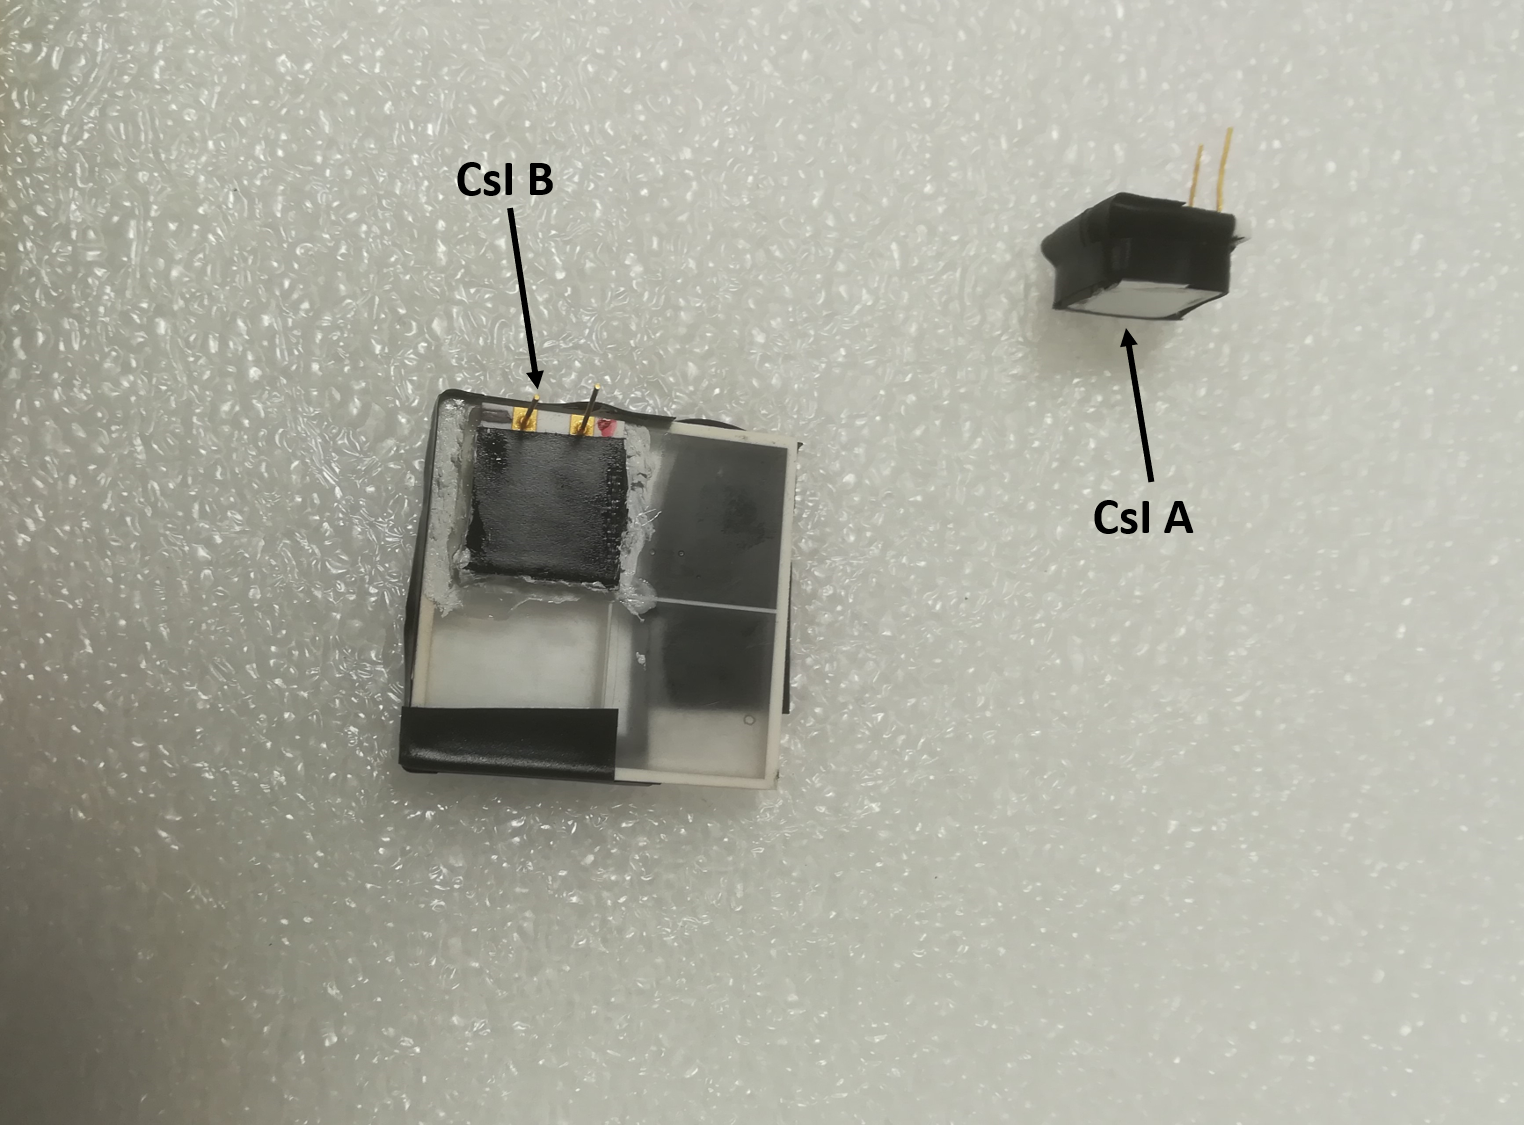
\includegraphics[width=\textwidth, keepaspectratio]{Grafici/csi_etichette.png}
	\caption{Gli scintillatori allo ioduro di cesio (CsI) utilizzati nel test: a sinistra il \emph{CsI~B}, a destra il \emph{CsI~A}.} \label{fig:csi}
\end{figure}




\begin{figure} [!t]
	\centering
	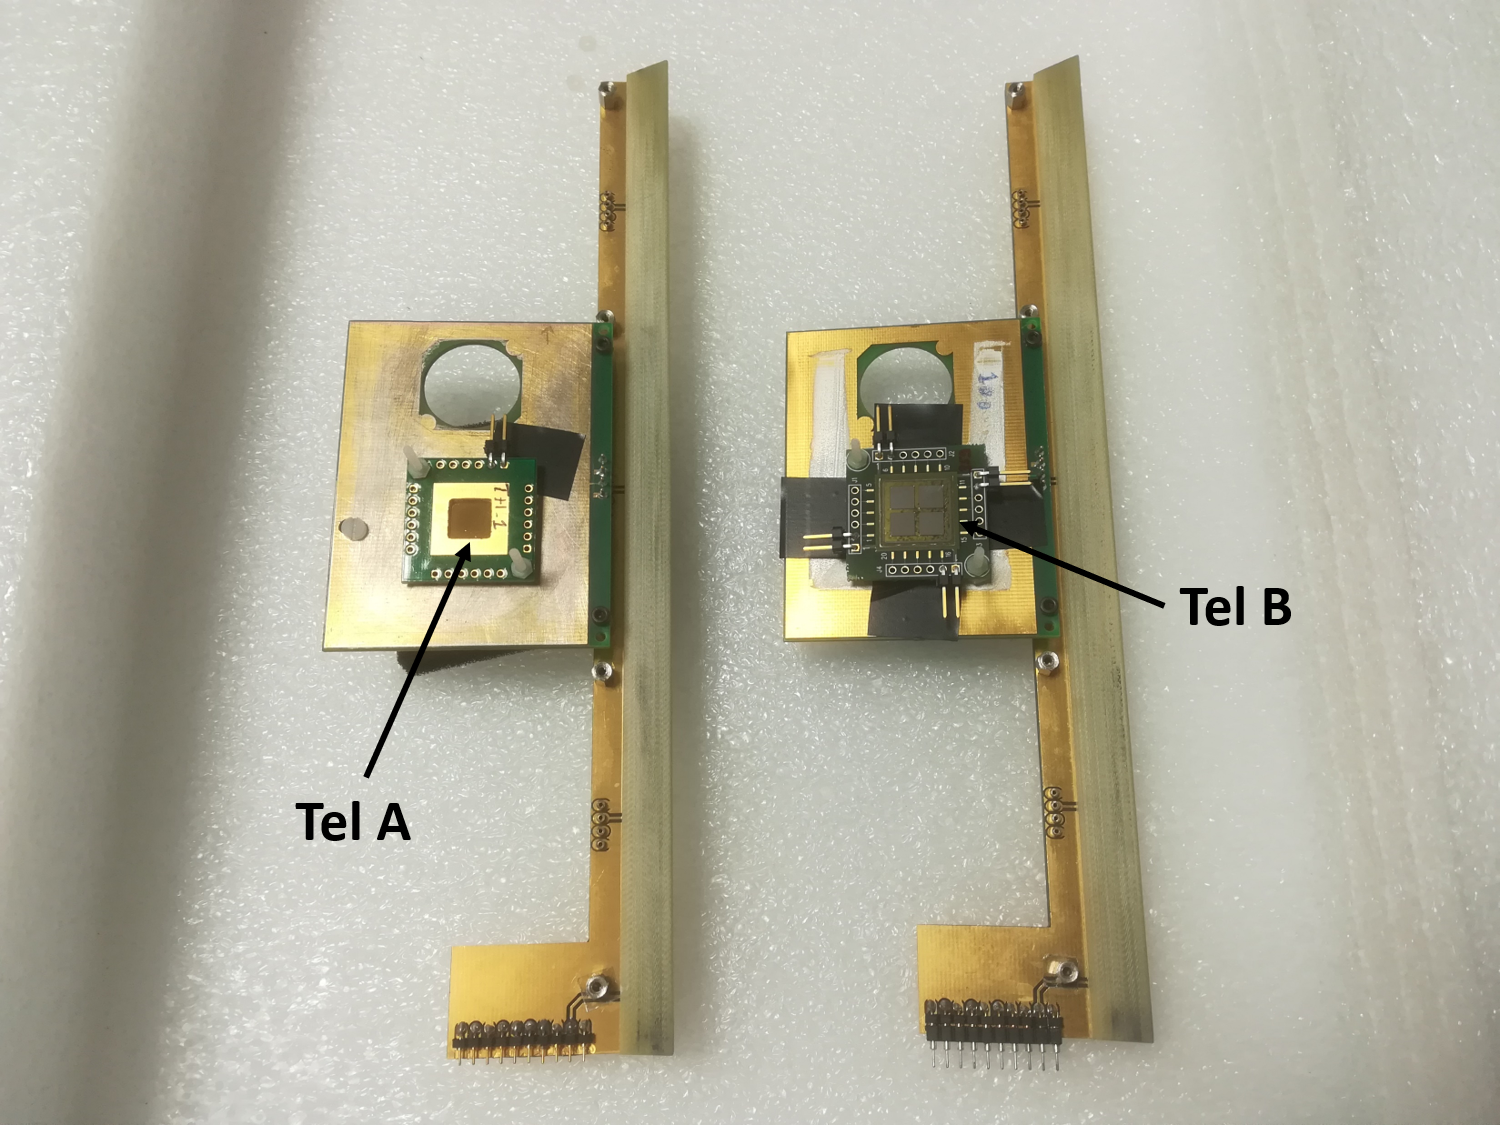
\includegraphics[width=\textwidth, keepaspectratio]{Grafici/telescopi_etichette.png}
	\caption{I due telescopi SiC-CsI utilizzati nel test: a sinistra il \emph{Tel~A}, a destra il \emph{Tel~B}.} \label{fig:telescopi}
\end{figure}



